\chapter{Resultados Experimentales, Regret Matching en Juegos en Forma Normal}
\label{apex:chapter:experimentos-rm}

En este apéndice se presentan las tablas y gráficas detalladas para los juegos en forma normal descritos en el capítulo \ref{chapter:regret-matching}. Para cada juego se muestra una tabla con la estrategia obtenida en la última corrida de cada uno de los procedimientos y, en caso de conocerse, el equilibrio de Nash. Para cada estrategia se muestra la utilidad de cada jugador si utilizan una mejor respuesta frente a la estrategia calculada para el oponente $v_1$ y $v_2$, así como la explotabilidad $\varepsilon_{\sigma}$ (ver la Sección \ref{chapter:explotabilidad} para definiciones formales).

Además, se presenta una tabla que indica el tiempo de cada ejecución ($T$), el número de iteraciones para alcanzar la cota deseada ($I$) y el tiempo promedio de cada iteración en cada una de las ejecuciones ($T/I$), así como el promedio del tiempo y del número de iteraciones para cada procedimiento. También se muestran las gráficas del regret por iteraciones, para observar su convergencia. Estas gráficas son mostradas con una escala logarítmica en el eje $x$ para apreciar mejor los resultados.

\newcommand{\graphicsRM}[2]{
\begin{figure}
    \caption{Gráficas del regret con respecto al número de iteraciones del juego #1}
    \label{fig:regret-#2}
    \centering
    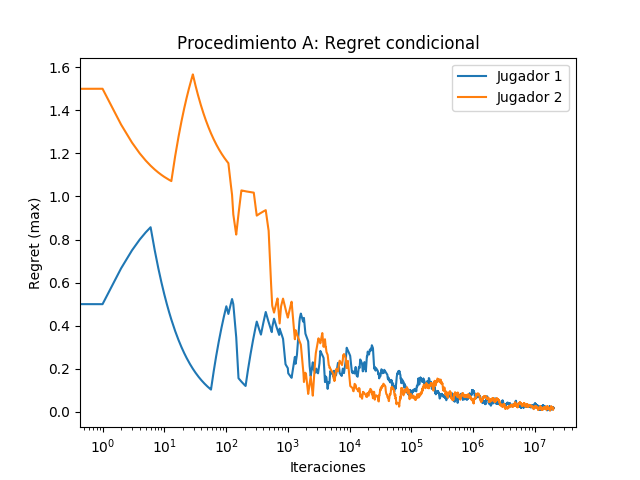
\includegraphics[width=0.58\textwidth]{graficas/#2/procedimiento-A.png}
    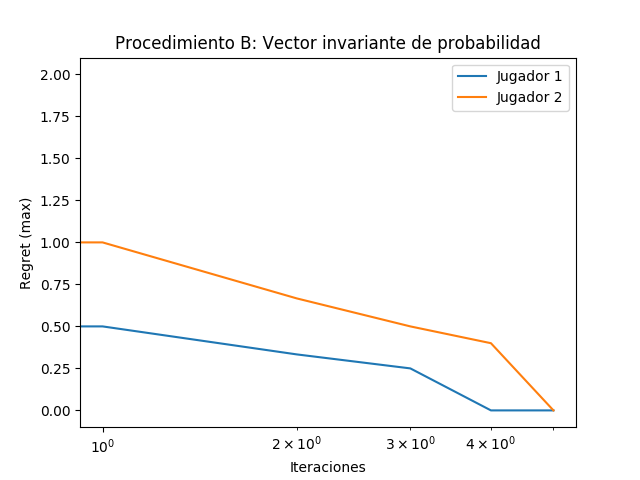
\includegraphics[width=0.58\textwidth]{graficas/#2/procedimiento-B.png}
    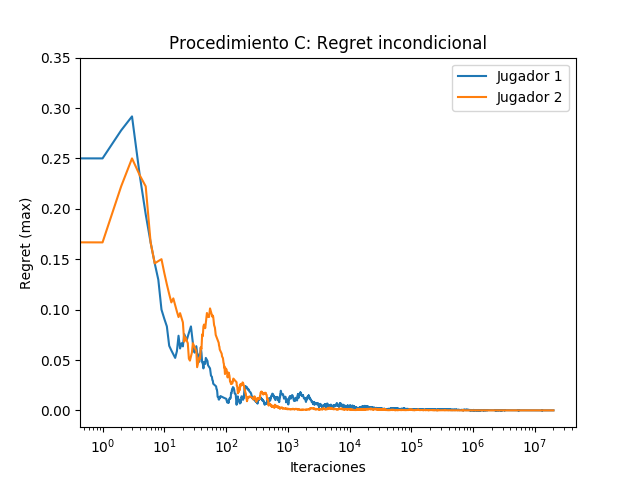
\includegraphics[width=0.58\textwidth]{graficas/#2/procedimiento-C.png}
\end{figure}
}

\section{Matching Pennies}

En este juego, si un jugador elige cada acción con una probabilidad de $0.5$, entonces su ganancia esperada es igual a $0$, sin importar la estrategia de su oponente, obteniendo el equilibrio de Nash cuando ambos jugadores utilizan esta estragia. Las estrategias obtenidas no corresponden al equilibrio de Nash, sin embargo, garantizan una utilidad cercana a $0$ en todos los casos, obteniendo una explotabilidad no mayor a $0.008$, como se muestra en la Tabla \ref{tab:estrategias-matching-pennies}. Por lo que todas las estrategias obtenidas son un $\varepsilon$- equilibrio de Nash, con $\varepsilon < 0.008$.

\begin{table}
    \centering
    \begin{tabular}{c|c|c|c|c}
    \hline
        & E.N. & A & B & C \\ \hline
        $\sigma_1$   & $(0.500, 0.500)$ & $(0.500, 0.500)$ & $(0.500, 0.500)$ & $(0.500,  0.500)$ \\
        $\sigma_2$   & $(0.500, 0.500)$ & $(0.497, 0.503)$ & $(0.503, 0.497)$ & $(0.504,  0.496)$ \\ \hline
        $(v_1, v_2)$ & $(0.000, 0.000)$ & $(0.006, 0.000)$ & $(0.006, 0.000)$ & $(0.008, 0.000)$ \\ \hline
        $\varepsilon_{\sigma}$ & $0$ & $0.006$ & $0.006$ & $0.008$ \\ \hline
    \end{tabular}
    \caption{Estrategias obtenidas del juego Matching Pennies}
    \label{tab:estrategias-matching-pennies}
\end{table}


La Tabla \ref{tab:resultados-matching-pennies} muestra los resultados obtenidos relacionados al tiempo y número de iteraciones de los procedimientos. El procedimiento A, regret condicional, tuvo una duración promedio de $10.276$ segundos, con un número promedio de iteraciones de $3892550.4$, obteniendo un promedio de $2.64 {\times} 10^{-6}$ segundos por iteración. Con el procedimiento B, que utiliza un vector invariante de probabilidad, se obtuvo un tiempo, número de iteraciones y tiempo por iteración promedios de $3.777$ segundos, $25616.6$ iteraciones y $3.03 {\times} 10^{-5}$ segundos por iteración, respectivamente. Por último, el procedimiento C, regret incondicional, se obtuvo un tiempo promedio de $0.042$, el número de iteraciones promedio fue de $16260.5$, obteniendo un promedio de $2.58 {\times} 10^{-6}$ segundos por iteración. 

\begin{table}
    \scriptsize
    \centering
    \begin{tabular}{r r r | r r r | r r r}
    \multicolumn{3}{c}{A} & \multicolumn{3}{c}{B} & \multicolumn{3}{c}{C} \\ \hline
    $T$ & $I$ & $T/I$ & $T$ & $I$ & $T/I$ & $T$ & $I$ & $T/I$ \\  \hline
	$7.663$ & $3068341$ & $2.50 {\times} 10^{-06}$ & $0.985$ & $32510$ & $3.03 {\times} 10^{-05}$ & $0.002$ & $955$ & $2.53 {\times} 10^{-06}$ \\
	$9.650$ & $3857071$ & $2.50 {\times} 10^{-06}$ & $1.748$ & $56946$ & $3.07 {\times} 10^{-05}$ & $0.064$ & $24968$ & $2.55 {\times} 10^{-06}$ \\
	$23.313$ & $8950013$ & $2.60 {\times} 10^{-06}$ & $0.552$ & $18401$ & $3.00 {\times} 10^{-05}$ & $0.061$ & $23854$ & $2.57 {\times} 10^{-06}$ \\
	$11.757$ & $4240611$ & $2.77 {\times} 10^{-06}$ & $0.309$ & $10197$ & $3.03 {\times} 10^{-05}$ & $0.025$ & $9724$ & $2.57 {\times} 10^{-06}$ \\
	$2.377$ & $877335$ & $2.71 {\times} 10^{-06}$ & $0.747$ & $24892$ & $3.00 {\times} 10^{-05}$ & $0.011$ & $4188$ & $2.59 {\times} 10^{-06}$ \\
	$5.062$ & $1818992$ & $2.78 {\times} 10^{-06}$ & $0.848$ & $28142$ & $3.01 {\times} 10^{-05}$ & $0.025$ & $9666$ & $2.60 {\times} 10^{-06}$ \\
	$4.281$ & $1557496$ & $2.75 {\times} 10^{-06}$ & $0.132$ & $4405$ & $3.01 {\times} 10^{-05}$ & $0.045$ & $16951$ & $2.64 {\times} 10^{-06}$ \\
	$22.110$ & $8230100$ & $2.69 {\times} 10^{-06}$ & $1.307$ & $43116$ & $3.03 {\times} 10^{-05}$ & $0.021$ & $8155$ & $2.64 {\times} 10^{-06}$ \\
	$3.691$ & $1432846$ & $2.58 {\times} 10^{-06}$ & $0.639$ & $21311$ & $3.00 {\times} 10^{-05}$ & $0.093$ & $35270$ & $2.64 {\times} 10^{-06}$ \\
	$12.853$ & $4892699$ & $2.63 {\times} 10^{-06}$ & $0.500$ & $16246$ & $3.08 {\times} 10^{-05}$ & $0.076$ & $28874$ & $2.64 {\times} 10^{-06}$ \\ \hline
	$10.276$ & $3892550.4$ & $2.64 {\times} 10^{-06}$ & $0.777$ & $25616.6$ & $3.03 {\times} 10^{-05}$ & $0.042$ & $16260.5$ & $2.58 {\times} 10^{-06}$ \\ \hline
    \end{tabular}
    \caption{Resultados del juego Matching Pennies}
    \label{tab:resultados-matching-pennies}
\end{table}

La Figura \ref{fig:regret-matching-pennies} muestra el regret incondicional con respecto al tiempo de la última corrida, para los $3$ procedimientos. Se observa que en todos los casos el \textit{regret} total de cada jugador converge a cero.

\graphicsRM{Matching Pennies}{matching-pennies}


\section{Piedra, Papel o Tijeras}

En este juego, al igual que en el anterior, ambos jugadores pueden garantizar una utilidad esperada de $0$ sin importar la estrategia utilizada por su oponente, que se obtiene al elegir cada acción con igual probabilidad. Las estrategias obtenidas son presentadas en la tabla \ref{tab:estrategias-RPS}. No todas corresponden al equilibrio de Nash exacto, sin embargo, cada una de ellas es un $\varepsilon$-equilibrio de Nash con $\varepsilon < 0.01$.

\begin{table}
    \centering
    \begin{tabular}{c c|c|r|r}
        \hline
        & & Estrategias & $v_1 / v_2$ & $\varepsilon_{\sigma}$ \\
        \hline
        \multirow{2}{*}{EN}
        & $\sigma_1$ & $(0.333, 0.333, 0.333)$ & $0.000$ & \multirow{2}{*}{$0.000$}\\
        & $\sigma_2$ & $(0.333, 0.333, 0.333)$ &  $0.000$ & \\
        \hline
        \multirow{2}{*}{A}
        & $\sigma_1$ & $(0.332, 0.335, 0.332)$ & $0.003$ & \multirow{2}{*}{$0.006$}\\
        & $\sigma_2$ & $(0.331, 0.334, 0.335)$ & $0.003$ & \\
        \hline
        \multirow{2}{*}{B}
        & $\sigma_1$ & $(0.330, 0.334, 0.336)$ & $0.006$ & \multirow{2}{*}{$0.010$}\\
        & $\sigma_2$ & $(0.329, 0.335, 0.337)$ & $0.004$ & \\
        \hline
        \multirow{2}{*}{C}
        & $\sigma_1$ & $(0.333, 0.337, 0.330)$ & $0.005$ & \multirow{2}{*}{$0.009$} \\
        & $\sigma_2$ &$(0.336, 0.330, 0.335)$  & $0.004$ & \\
        \hline
    \end{tabular}
    \caption{Estrategias obtenidas del juego Piedra, Papel o Tijeras}
    \label{tab:estrategias-RPS}
\end{table}

La Tabla \ref{tab:resultados-RPS} muestra los resultados obtenidos relacionados al tiempo y número de iteraciones de los procedimientos. El procedimiento A, \textit{regret} condicional, tuvo una duración promedio de $25.715$ segundos, con un número promedio de iteraciones de $4519054.1$, obteniendo un promedio de $2.7 {\times} 10^{-6}$ segundos por iteración. Con el procedimiento B, que utiliza un vector invariante de probabilidad, se obtuvo un tiempo, número de iteraciones y tiempo por iteración promedios de $0.345$ segundos, $6601.3$ iteraciones y $5.23 {\times} 10^{-5}$ segundos por iteración, respectivamente. Por último, el procedimiento C, \textit{regret} incondicional, se obtuvo un tiempo promedio de $0.049$, el número de iteraciones promedio fue de $19321.1$, obteniendo un promedio de $2.54 {\times} 10^{-6}$ segundos por iteración.

\begin{table}
    \scriptsize
    \centering
    \begin{tabular}{r r r | r r r | r r r}
    \multicolumn{3}{c}{A} & \multicolumn{3}{c}{B} & \multicolumn{3}{c}{C} \\ \hline
    $T$ & $I$ & $T/I$ & $T$ & $I$ & $T/I$ & $T$ & $I$ & $T/I$ \\  \hline
    $25.715$ & $9107389$ & $2.82 {\times} 10^{-06}$ & $0.724$ & $13750$ & $5.26 {\times} 10^{-05}$ & $0.034$ & $12967$ & $2.64 {\times} 10^{-06}$ \\
    $29.494$ & $10951479$ & $2.69 {\times} 10^{-06}$ & $0.692$ & $13257$ & $5.22 {\times} 10^{-05}$ & $0.041$ & $16096$ & $2.57 {\times} 10^{-06}$ \\
    $7.015$ & $2641656$ & $2.66 {\times} 10^{-06}$ & $0.000$ & $6$ & $4.36 {\times} 10^{-05}$ & $0.063$ & $24423$ & $2.56 {\times} 10^{-06}$ \\
    $4.610$ & $1748365$ & $2.64 {\times} 10^{-06}$ & $0.849$ & $16255$ & $5.22 {\times} 10^{-05}$ & $0.048$ & $18613$ & $2.56 {\times} 10^{-06}$ \\
    $8.051$ & $3033028$ & $2.65 {\times} 10^{-06}$ & $0.000$ & $3$ & $4.28 {\times} 10^{-05}$ & $0.082$ & $32222$ & $2.55 {\times} 10^{-06}$ \\
    $9.870$ & $3717278$ & $2.66 {\times} 10^{-06}$ & $0.000$ & $3$ & $4.28 {\times} 10^{-05}$ & $0.084$ & $33042$ & $2.54 {\times} 10^{-06}$ \\
    $2.749$ & $1037895$ & $2.65 {\times} 10^{-06}$ & $0.000$ & $3$ & $4.06 {\times} 10^{-05}$ & $0.049$ & $19316$ & $2.55 {\times} 10^{-06}$ \\
    $11.971$ & $4517546$ & $2.65 {\times} 10^{-06}$ & $0.556$ & $10644$ & $5.23 {\times} 10^{-05}$ & $0.024$ & $9601$ & $2.54 {\times} 10^{-06}$ \\
    $14.974$ & $5606070$ & $2.67 {\times} 10^{-06}$ & $0.000$ & $3$ & $3.74 {\times} 10^{-05}$ & $0.014$ & $5621$ & $2.55 {\times} 10^{-06}$ \\
    $7.532$ & $2829835$ & $2.66 {\times} 10^{-06}$ & $0.631$ & $12089$ & $5.22 {\times} 10^{-05}$ & $0.054$ & $21310$ & $2.55 {\times} 10^{-06}$ \\ \hline
    $12.198$ & $4519054.1$ & $2.70 {\times} 10^{-06}$ & $0.345$ & $6601.3$ & $5.23 {\times} 10^{-05}$ & $0.049$ & $19321.1$ & $2.54 {\times} 10^{-06}$ \\ \hline
    \end{tabular}
    \caption{Resultados del juego Piedra, Papel o Tijeras}
    \label{tab:resultados-RPS}
\end{table}

La Figura \ref{fig:regret-RPS} muestra el regret incondicional con respecto al tiempo de la última corrida para los procedimientos A, B y C. Se observa como el \textit{regret} total de ambos jugadores converge a cero.

\graphicsRM{Piedra, Papel o Tijeras}{RPS}

\section{Ficha vs. Dominó}

El primer jugador puede garantizar una ganancia esperada de, al menos $1/3$, por lo que el segundo jugador puede garantizar no perder más de $1/3$. A diferencia de los juegos anteriores, la matriz de pagos de este juegos no es simétrica y el primer jugador tiene ventaja sobre el segundo. Además, este juego no tiene un equilibrio de Nash único. En la Tabla \ref{tab:estrategias-RPS} se observa que las estrategias obtenidas para el primer jugador le permiten obtener una ganancia esperada al menos de $0.330$, $0.326$ y $0.329$, respectivamente para los procedimientos A, B y C. Todos estos valores son menores que $1/3$, pero con una diferencia menor que $0.01$. Por otra parte el segundo jugador puede garantizar un valor esperado no menor que $-0.338$ con cualquiera de los procedimientos.

\begin{table}
    \centering
    \begin{tabular}{c c|c|r|r}
        \hline
        & & Estrategias & $v_1 / v_2$ & $\varepsilon_{\sigma}$ \\
        \hline
        \multirow{2}{*}{EN}
        & $\sigma_1$ & $(0.333, 0.333, 0.000, 0.000, 0.000, 0.000, 0.333)$ & $0.333$ & \multirow{2}{*}{$0.000$}\\
        & $\sigma_2$ & $(0.333, 0.000, 0.333, 0.000, 0.333, 0.000)$ &  $-0.333$ & \\
        \hline
        \multirow{2}{*}{A}
        & $\sigma_1$ & $(0.136, 0.137, 0.116, 0.118, 0.198, 0.081, 0.214)$ & $0.338$ &\multirow{2}{*}{$0.010$} \\
        & $\sigma_2$ & $(0.165, 0.171, 0.163, 0.166, 0.166, 0.169)$ & $-0.328$ &\\
        \hline
        \multirow{2}{*}{B}
        & $\sigma_1$ & $(0.121, 0.118, 0.135, 0.137, 0.214, 0.078, 0.198)$ & $0.335$ & \multirow{2}{*}{$0.007$} \\
        & $\sigma_2$ & $(0.157, 0.178, 0.156, 0.177, 0.157, 0.175)$ & $-0.331$ & \\
        \hline
        \multirow{2}{*}{C}
        & $\sigma_1$ & $(0.128, 0.128, 0.129, 0.134, 0.208, 0.073, 0.202)$ & $0.334$ & \multirow{2}{*}{$0.004$} \\
        & $\sigma_2$ & $(0.169, 0.165, 0.168, 0.164, 0.169, 0.165)$ & $-0.330$ & \\
        \hline
    \end{tabular}
    \caption{Estrategias obtenidas del juego Ficha vs Dominó}
    \label{tab:estrategias-domino}
\end{table}

La Tabla \ref{tab:resultados-domino} muestra los resultados obtenidos relacionados al tiempo y número de iteraciones de los procedimientos de este juego. El procedimiento A, regret condicional, tuvo una duración promedio de $319.179$ segundos, con un número promedio de iteraciones de $108319272.4$, obteniendo un promedio de $2.95 {\times} 10^{-6}$ segundos por iteración. Con el procedimiento B, que utiliza un vector invariante de probabilidad, se obtuvo un tiempo, número de iteraciones y tiempo por iteración promedios de $11.275$ segundos, $75250.2$ iteraciones y $1.5 {\times} 10^{-4}$ segundos por iteración, respectivamente. Por último, el procedimiento C, regret incondicional, se obtuvo un tiempo promedio de $0.237$, el número de iteraciones promedio fue de $84318.5$, obteniendo un promedio de $2.81 {\times} 10^{-6}$ segundos por iteración. 

\begin{table}
   \scriptsize
    \centering
    \begin{tabular}{r r r | r r r | r r r}
    \multicolumn{3}{c}{A} & \multicolumn{3}{c}{B} & \multicolumn{3}{c}{C} \\ \hline
    $T$ & $I$ & $T/I$ & $T$ & $I$ & $T/I$ & $T$ & $I$ & $T/I$ \\  \hline
	$669.839$ & $215859538$ & $3.10 {\times} 10^{-06}$ & $4.458$ & $29721$ & $1.50 {\times} 10^{-04}$ & $0.188$ & $66700$ & $2.81 {\times} 10^{-06}$ \\
	$309.685$ & $117568373$ & $2.63 {\times} 10^{-06}$ & $9.019$ & $60333$ & $1.49 {\times} 10^{-04}$ & $0.260$ & $92401$ & $2.82 {\times} 10^{-06}$ \\
	$399.170$ & $152612646$ & $2.62 {\times} 10^{-06}$ & $3.646$ & $24338$ & $1.50 {\times} 10^{-04}$ & $0.212$ & $75674$ & $2.81 {\times} 10^{-06}$ \\
	$131.570$ & $38097125$ & $3.45 {\times} 10^{-06}$ & $12.996$ & $86898$ & $1.50 {\times} 10^{-04}$ & $0.145$ & $51776$ & $2.80 {\times} 10^{-06}$ \\
	$263.482$ & $96741015$ & $2.72 {\times} 10^{-06}$ & $4.516$ & $30170$ & $1.50 {\times} 10^{-04}$ & $0.134$ & $47862$ & $2.80 {\times} 10^{-06}$ \\
	$203.854$ & $77156602$ & $2.64 {\times} 10^{-06}$ & $15.420$ & $103021$ & $1.50 {\times} 10^{-04}$ & $0.385$ & $136950$ & $2.81 {\times} 10^{-06}$ \\
	$201.267$ & $76467409$ & $2.63 {\times} 10^{-06}$ & $17.399$ & $115935$ & $1.50 {\times} 10^{-04}$ & $0.351$ & $124882$ & $2.81 {\times} 10^{-06}$ \\
	$316.007$ & $97849871$ & $3.23 {\times} 10^{-06}$ & $17.266$ & $115056$ & $1.50 {\times} 10^{-04}$ & $0.203$ & $72315$ & $2.81 {\times} 10^{-06}$ \\
	$383.736$ & $110341861$ & $3.48 {\times} 10^{-06}$ & $12.805$ & $85532$ & $1.50 {\times} 10^{-04}$ & $0.271$ & $96438$ & $2.81 {\times} 10^{-06}$ \\
	$313.177$ & $100498284$ & $3.12 {\times} 10^{-06}$ & $15.227$ & $101498$ & $1.50 {\times} 10^{-04}$ & $0.220$ & $78187$ & $2.81 {\times} 10^{-06}$ \\ \hline
	$319.179$ & $108319272.4$ & $2.95 {\times} 10^{-06}$ & $11.275$ & $75250.2$ & $1.50 {\times} 10^{-04}$ & $0.237$ & $84318.5$ & $2.81 {\times} 10^{-06}$ \\ \hline
    \end{tabular}
    \caption{Resultados del juego Ficha vs Dominó}
    \label{tab:resultados-domino}
\end{table}

\graphicsRM{Ficha vs. Dominó}{domino}

La Figura \ref{fig:regret-domino} muestra el regret incondicional con respecto al tiempo de la última corrida, para los procedimientos A, B y C. Se observa como el \textit{regret} máximo converge a cero para ambos jugadores en cada uno de los procedimientos.



\section{Coronel Blotto}

En este juego no se posee un equilibrio de Nash como referencia. Sin embargo, como la matriz de pagos es simétrica, el valor del juego debe ser $0$, así que las estrategias obtenidas, se mostradas en la Tabla \ref{tab:estrategias-coronel-blotto}, deben garantizar un valor esperado cercano a $0$. En esta tabla, también se observa que cada una de las estrategias tienen una explotabilidad menor o igual que $0.011$.

\begin{table}
    \scriptsize
    \centering
    \begin{tabular}{c}
        Estrategias \\
        \hline
        Procedimiento A \\ \hline
         $(0, 0, 0.126, 0.113, 0, 0, 0, 0.080, 0, 0.100, 0, 0.131, 0, 0.001, 0.111, 0.118, 0.094, 0.124, 0, 0, 0)$ \\
         $(0, 0, 0.101, 0.109, 0, 0, 0, 0.116, 0, 0.139, 0, 0.132, 0, 0.002, 0.076, 0.076, 0.141, 0.106, 0, 0, 0)$ \\
         $(v_1, v_2) = (0.002, 0.008)$ \\
         $\varepsilon_{\sigma} = 0.01$ \\
        \hline
        Procedimiento B \\ \hline
         $(0, 0.002, 0.093, 0.110, 0.001, 0, 0.002, 0.111, 0.001, 0.128, 0.001, 0.126, 0, 0.001, 0.076, 0.112, 0.088, 0.145, 0.001, 0.001, 0)$ \\
         $(0, 0.001, 0.102, 0.107, 0.001, 0, 0.0, 0.154, 0.001, 0.099, 0, 0.055, 0.001, 0, 0.156, 0.113, 0.140, 0.069, 0.002, 0.001, 0)$ \\
         $(v_1, v_2) = (0.004, 0.007)$ \\
         $\varepsilon_{\sigma} = 0.011$ \\
        \hline
        Procedimiento C \\ \hline
         $(0, 0, 0.119, 0.106, 0, 0, 0, 0.110, 0, 0.107, 0, 0.108, 0, 0, 0.122, 0.122, 0.117, 0.1, 0, 0, 0)$ \\
         $(0, 0, 0.148, 0.096, 0, 0, 0, 0.099, 0, 0.095, 0, 0.093, 0, 0, 0.155, 0.126, 0.117, 0.070, 0, 0, 0)$ \\
         $(v_1, v_2) = (0.004, 0.005)$ \\
         $\varepsilon_{\sigma} = 0.009$ \\
        \hline
    \end{tabular}
    \caption{Estrategias obtenidas del juego Coronel Blotto}
    \label{tab:estrategias-coronel-blotto}
\end{table}

Los resultados obtenidos relacionados al tiempo y número de iteraciones de cada procedimiento son mostrados en la Tabla \ref{tab:resultados-coronel-blotto}.

\begin{table}
   \scriptsize
    \centering
    \begin{tabular}{r r r | r r r | r r r}
    \multicolumn{3}{c}{A} & \multicolumn{3}{c}{B} & \multicolumn{3}{c}{C} \\ \hline
    $T$ & $I$ & $T/I$ & $T$ & $I$ & $T/I$ & $T$ & $I$ & $T/I$ \\  \hline
	$940.377$ & $197127165$ & $4.77 {\times} 10^{-06}$ & $90.239$ & $75420$ & $1.20 {\times} 10^{-03}$ & $0.047$ & $13559$ & $3.50 {\times} 10^{-06}$ \\
	$532.020$ & $109697363$ & $4.85 {\times} 10^{-06}$ & $74.886$ & $62704$ & $1.19 {\times} 10^{-03}$ & $0.192$ & $56383$ & $3.41 {\times} 10^{-06}$ \\
	$396.583$ & $82924728$ & $4.78 {\times} 10^{-06}$ & $56.735$ & $47416$ & $1.20 {\times} 10^{-03}$ & $0.046$ & $13664$ & $3.39 {\times} 10^{-06}$ \\
	$362.203$ & $80521418$ & $4.50 {\times} 10^{-06}$ & $41.290$ & $34596$ & $1.19 {\times} 10^{-03}$ & $0.162$ & $47742$ & $3.40 {\times} 10^{-06}$ \\
	$967.890$ & $207963652$ & $4.65 {\times} 10^{-06}$ & $69.359$ & $58123$ & $1.19 {\times} 10^{-03}$ & $0.090$ & $26547$ & $3.40 {\times} 10^{-06}$ \\
	$1016.540$ & $245737655$ & $4.14 {\times} 10^{-06}$ & $64.457$ & $53560$ & $1.20 {\times} 10^{-03}$ & $0.118$ & $34715$ & $3.41 {\times} 10^{-06}$ \\
	$553.971$ & $112170109$ & $4.94 {\times} 10^{-06}$ & $80.789$ & $67624$ & $1.19 {\times} 10^{-03}$ & $0.261$ & $76657$ & $3.40 {\times} 10^{-06}$ \\
	$966.339$ & $204832370$ & $4.72 {\times} 10^{-06}$ & $138.294$ & $115846$ & $1.19 {\times} 10^{-03}$ & $0.358$ & $105149$ & $3.40 {\times} 10^{-06}$ \\
	$1787.020$ & $384044065$ & $4.65 {\times} 10^{-06}$ & $84.924$ & $70978$ & $1.20 {\times} 10^{-03}$ & $0.121$ & $35434$ & $3.42 {\times} 10^{-06}$ \\
	$1232.380$ & $277204528$ & $4.45 {\times} 10^{-06}$ & $92.610$ & $77517$ & $1.19 {\times} 10^{-03}$ & $0.260$ & $76285$ & $3.41 {\times} 10^{-06}$ \\ \hline
	$875.533$ & $190222305.3$ & $4.60 {\times} 10^{-06}$ & $79.358$ & $66378.4$ & $1.20 {\times} 10^{-03}$ & $0.166$ & $48613.5$ & $3.41 {\times} 10^{-06}$ \\ \hline
    \end{tabular}
    \caption{Resultados del juego Coronel Blotto}
    \label{tab:resultados-coronel-blotto}
\end{table}

 El procedimiento A, regret condicional, tuvo una duración promedio de $875.533$ segundos, con un número promedio de iteraciones de $190222305.3$, obteniendo un promedio de $4.60 {\times} 10^{-6}$ segundos por iteración. Con el procedimiento B, que utiliza un vector invariante de probabilidad, se obtuvo un tiempo, número de iteraciones y tiempo por iteración promedios de $79.358$ segundos, $66378.4$ iteraciones y $1.2 {\times} 10^{-3}$ segundos por iteración, respectivamente. Por último, el procedimiento C, regret incondicional, se obtuvo un tiempo promedio de $0.166$, el número de iteraciones promedio fue de $48613.5$, obteniendo un promedio de $3.41 {\times} 10^{-6}$ segundos por iteración.
 
 \graphicsRM{Coronel Blotto}{coronel-blotto}
 
 La Figura \ref{fig:regret-coronel-blotto} muestra el regret incondicional con respecto al tiempo de la última corrida para los tres procedimientos. Se observa que el regret máximo tiende a cero para cada uno de los jugadores en todos los procedimientos.
 